\documentclass[12pt,a4paper]{article}
\usepackage{ucs}
\usepackage[utf8x]{inputenc}
\usepackage{amsmath}
\usepackage{graphicx}
\usepackage{wrapfig}
\usepackage{trfsigns}
\usepackage{xfrac}

\title{Osnove Mehatronike 5. lab}
\newcommand{\brvjezbe}{3}
\newcommand{\ime}{Niko Višnjić}
\newcommand{\jmbag}{0036449299}
\newcommand{\grupa}{unknown}
\newcommand{\predmet}{Osnove mehatronike} 
\newcommand{\fakultet}{Fakultet elektrotehnike i računarstva Zagreb} 
\newcommand{\zavod}{Zavod za elektrostrojarstvo i automatizaciju } 
\newcommand{\imevjezbe}{Vježba 5: Regulacija pozicije rotacijskog elektromehaničkog sustava SRV02 
\newline-sinteza regulatora-}
\usepackage[hmargin={3.5cm,2.5cm},height=25.5cm]{geometry}
\input{"zaglavlje.tex"}
\setcounter{secnumdepth}{4}

\DeclareMathSizes{12}{12}{10}{12}

\begin{document}
\section{Uvod}
U okviru ove vježbe obavljamo pokus koji obuhvaća proces implementacije
(rad u realnom vremenu) regulatora pozicije projektiranog i simuliranog sustava tokom četvrte laboratorijske vježbe. 

Koristi se Simulink/WinCon okruženje kao programski razvojni alat. Postupak provjere obuhvaća usporedbu dobivenih rezultata testiranja s rezultatima dobivenim simulacijom rotacijskog modula SRV02 te s regulacijskim zahtjevima postavljenim u vježbi 4.

U nastavku dokumentiramo i opisujemo pokuse te bilježimo dobivene rezultate i naša zapažanja iz dobivenih mjerenja.

\newpage


\section{Pokusi}
\subsection{Pokus 1: Implementacija i provjera sinteze regulatora pozicije rotacijskog elektromehaničkog sustava SRV02}

U sklopu ovog pokusu se implementira regulator pozicije rotacijskog elektromehaničkog sustava SRV02. 

Zadatak je korištenjem Simulink-a načiniti algoritam za regulaciju pozicije rotacijskog elektromehaničkog sustava SRV02 u realnom vremenu, korištenjem Real Time Windows Target okruženja testirati te provjeriti da li se 
regulacijske karakteristike kruga podudaraju sa zadanim regulacijskim zahtjevima
(definirani u vježbi 4.) te usporediti dzive realnog i simuliranog sustava regulacije pozicije.

\subsection{Shema spajanja realnog sustava i upravljački algoritam}

Kako bi mogli upravljati našim realnim rotacijskim modulom SRV02 i povezati isti s MATLAB-om radi mjerenja vrijednosti, potrebno je spojiti isti kao što je prikazano na slici 2.1.

\begin{figure}[h]
	\begin{center}
	\includegraphics[width=0.8\textwidth] {shema_spoj.png}
    \caption{Shema spoja za implementaciju regulatora pozicije na realni elektromehanički sustav}
    \end{center}
\end{figure}

Na temelju sinteze regulatora provedene u vježbi 4., potrebno je izraditi algoritam regulacije pozicije. Zbog potrebe usporedbe realnog i simuliranog odziva pozicije modula, u sklopu iste datoteke potrebno je izraditi i simulacijski model. Referentna vrijednost pozicije zadaje se programski. Ona je zajednička za simulacijski dio i za dio algoritma koji upravlja realnim sustavom (SRV02). Nadomjesnu shemu upravljačkog algoritma prilagođenu za korištenje u MATLAB/Simulink okruženju možemo vidjeti na slici 2.2.

\begin{figure}[h]
	\begin{center}
	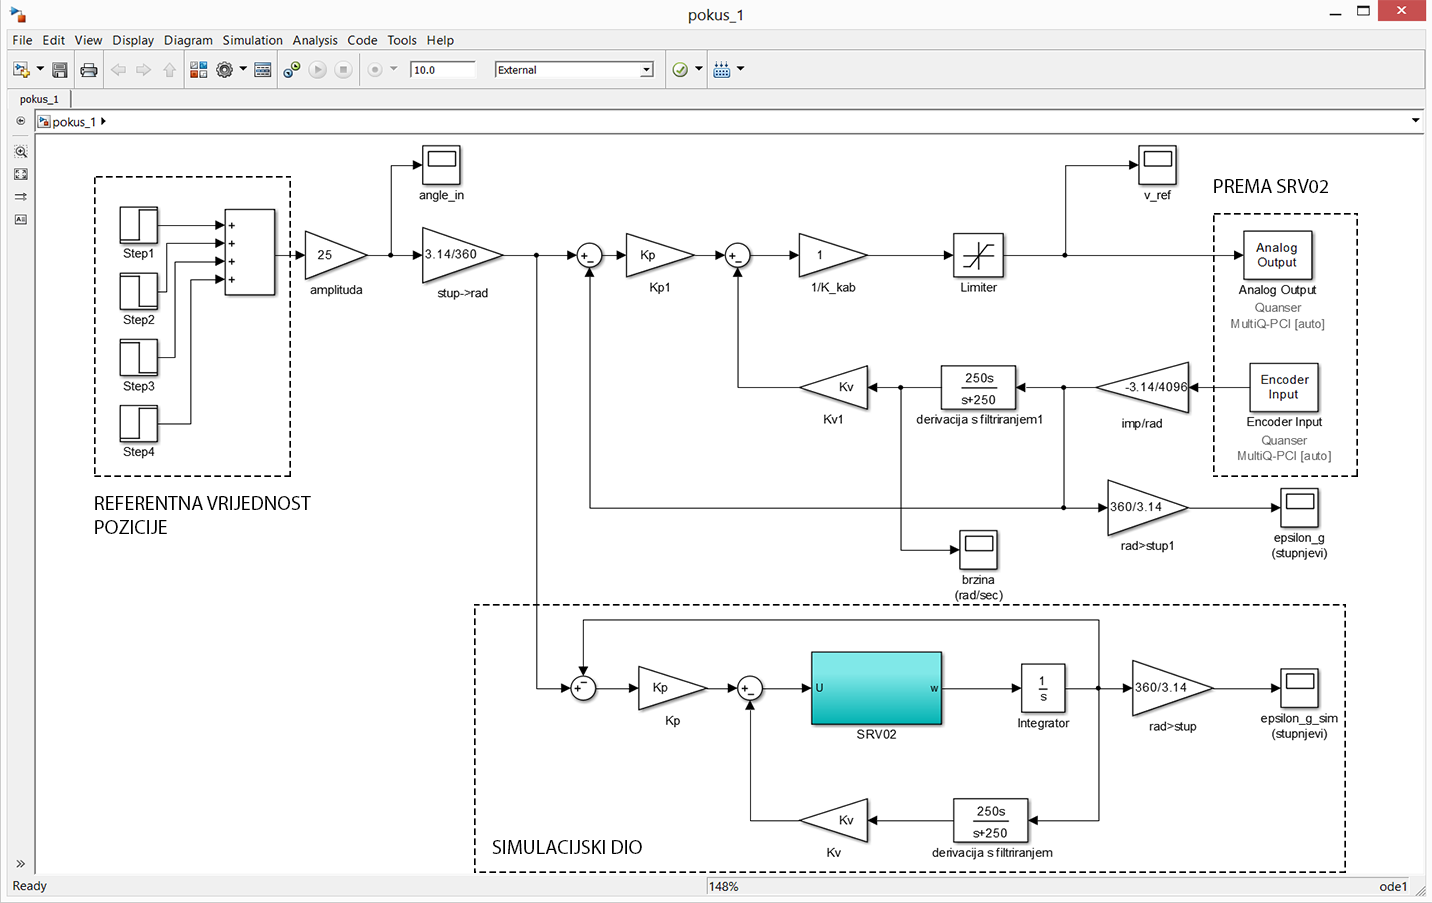
\includegraphics[width=0.8\textwidth] {model_oznake.png}
    \caption{Nadomjesna shema upravljačkog algoritma u Simulink okruženju}
    \end{center}
\end{figure}

Simulacijski model je identičan modelu u vježbi 4. 

Većina korištenih blokova u simulacijskom i realnom dijelu upravljačkog algoritma je identična. Jedina razlika je u tome što se u realnom dijelu upravljačkog algoritma umjesto SRV02 simulacijskog modela koristi realni proces, elektromehanički modul SRV02. Veza tog realnog procesa s ostalim dijelovima sustava regulacije odvija se preko ulazno-izlaznog sučelja. U ovom slučaju to su jedan analogni izlaz i jedan analogni ulaz. Analogni izlaz prosljeđuje
upravljački signal prema energetskom pojačalu modula SRV02, dok se pomoću analognog ulaza prosljeđuje informacija s enkodera prema upravljačkom algoritmu.

Provjera regulacijskih karakteristika vrši se snimanjem odziva pozicije osovine na skokovitu promjenu referentne veličine. Potrebno je snimiti odtiv sustava na test ulaznu funkciju oblika prikazanog na slici 2.3.


\begin{figure}[h]
	\begin{center}
	\includegraphics[width=0.8\textwidth] {ref.png}
    \caption{Odziv funkcije referentnog signala sustava}
    \end{center}
\end{figure}

\newpage

\subsection{Rezultati mjerenja i simulacije}

Izvođenjem našeg algoritma upravljanja na realan model, odnosno simulacijom za zadani regulator na matematičkom modelu dobivamo sljedeće odzive.

\begin{figure}[h]
	\begin{center}
	\includegraphics[width=0.8\textwidth, height = 3.5in]{odziv_ref_sim_real.png}
    \caption{Odziv simuliranog i mjerenog sustava na referentni signal pozicije}
    \end{center}
\end{figure}

Na slici 2.4 imamo istovremeno prikazane izmjerene vrijednosti realnog sustava te odzive simuliranog sustava i referentnog upravljačkog signala. Isti odziv, pri rastućem bridu referentnog signala, možemo pobliže vidjeti na slici 2.5.

\begin{figure}[h!]
	\begin{center}
	\includegraphics[width=0.8\textwidth, height = 3.5in] {odziv_ref_sim_real_close.png}
    \caption{Odziv simuliranog i mjerenog sustava na referentni signal pozicije, uvećani prikaz}
    \end{center}
\end{figure}

\newpage

Primjećujemo da odziv mjerenog realnog sustava nema nadvišenje koje imamo kod odziva simuliranog sustav. To je posljedica zanemarenja, odnosno simplifikacija, koje smo napravili prilikom modeliranja našeg matematičkog modela realnog sustava. Ukoliko promatramo detalje prijelazne pojave ovog odaziva, sl. 2.6., primjećujemo da nakon ustaljenja vrijednosti i realnog i simuliranog sustava postoji zamjetno odstupanje realnog sustava od referentne vrijednosti. To statičko odstupanje je posljedica zanemarenja koje smo učinili te mehaničkih i električkih svojstva realnog SRV02 modula, od kojih su najizraženija električka neosjetljivost motora SRV02 modula na male promjene upravljačkog napona, odnosno pozicije, te integralno djelovanje samog SRV02 modula. Ta odstupanja trebamo imati na umu pri korištenju vrijednosti dobivenih simulacijom, no ista nisu toliko velika u usporedbi s amplitudom referentnog signala da bi smatrali simulacijom netočnom.

\begin{figure}[h]
	\begin{center}
	\includegraphics[width=0.8\textwidth] {odziv_ref_sim_real_closer.png}
    \caption{Odziv simuliranog i mjerenog sustava na referentni signal pozicije, uvećani prikaz}
    \end{center}
\end{figure}

Kako bi usporedili dinamička svojstva SRV02 modula treba pogledati i usporediti odzive pozicije te odzive brzine vrtnje za dati realan sustav. Iste možemo vidjeti na slikama 2.7 i 2.8.

\newpage

\begin{figure}[ht!]
	\begin{center}
	\includegraphics[width=0.8\textwidth] {odziv_spd_pos.png}
    \caption{Odziv pozicije i brzine vrtnje realnog sustava SRV02}
    \end{center}
\end{figure}


\begin{figure}[hb!]
	\begin{center}
	\includegraphics[width=0.8\textwidth] {spd_pos_close.png}
    \caption{Odziv pozicije i brzine vrtnje realnog sustava SRV02, uvećani prikaz}
    \end{center}
\end{figure}

\newpage

\subsection{Opažanja i zaključci}

Usporedbom dobivenih odziva realnog i simuliranog sustava možemo zaključiti da oba sustava dovoljno dobro prate regulacijske zahtjeve zadane u sklopu četvrte laboratorijske vježbe, iako ne i jednako dobro. Ta razlika je posljedica nesavršenosti našeg matematičkog modela kojeg smo s namjernom simplificirali radi lakšeg modeliranja PV regulatora te iako su unapređenja i prilagođavanje istoga realnom sustavu moguća, za potrebe ove vježbe su suvišna.

Usporedimo li graničnu frekvenciju zatvorenog kruga regulacije pozicije te graničnu frekvenciju zatvorenog kruga regulacije brzine vrtnje, koje su iznosa 
$\omega_b = 44.36 \;rad/s$, odnosno $\omega_b = 139.28 \; rad/s$, možemo primjetiti zamjetnu razliku. Ista je posljedica odnosa između granične frekvencije i vremena prvog maksimuma. Kako su postavljeni različiti regulacijski zahtjevi, odnosno vremena prvog maksimuma, kod dva konfigurirana regulatora, tako se i granične frekvencije razlikuju.

U ovoj vježbi korišteni mjerni član na SRV02 modulu je enkoder kojega spajamo direktno na digitalni ulaz. Kako enkoder kao svoj izlaz šalje digitalne impulse koji broje pomake sustava uzlazno, odnosno silazno, ovisno o smjeru rotacije SRV02 modula, isti signal moramo derivirati kako bi dobili brzinu vrtnje. Ukoliko pogledamo odzive na slikama 2.7 i 2.8 možemo primjetiti da derivacijom istoga dobivamo isprekidanu, odnosno nazubljenu krivulju, koja je posljedica inherentne diskretnosti enkoderskog signala,. Potencijalno rješenje tog problema je da umjesto digitalnog enkodera koristimo tahnogenerator kao analogni izlaz sustava SRV02. Ukoliko koristimo tahogenerator za očitanje brzine vrtnje, nije potrebno derivirati ulazni analogni signal nakon diskretizacije, nego nam isti direktno daje informaciju o brzini vrtnje rotacijskog modula SRV02. Naravno, s obzirom na karakteristike tahogeneratora, njegov ulazni signal moramo skalirati s koeficijentom $\sfrac{1000}{1.5}$ da bi dobili vrijednost brzine vrtnje u okretajima u minuti.
Također, zbog toga što tahogenerator direktno očitava brzinu vrtnje motora, a nas zanima brzina vrtnje pogonske osovine, moramo dodatno dijeliti brzinu vrtnje s iznosom prijenosnog omjera $K_g = 70$. Time smo eliminirali derivator i dobili puno zaglađeniju regulaciju pozicije SRV02 modula.


\end{document}




%Na vlastitu odgovornost...